\begin{frame}
    \frametitle{Simulation - 1 server}
    \centering

    \begin{figure}[h]
        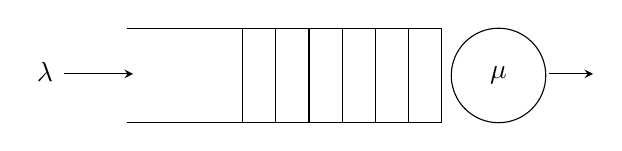
\begin{tikzpicture}[>=stealth, scale=0.8] 
            \draw (2,1.25) -- ++(5cm,0) -- ++(0,-1.5cm) -- ++(-5cm,0);
            \foreach \i in {1,...,6}
            \draw (7cm-\i*15pt,1.25) -- +(0,-1.5cm);
            \draw (7.9,0.5) circle [radius=0.75cm];
            \node[] at (0.7, 0.55) {$\lambda$};
            \draw[->] (1, 0.525) -- (2.1, 0.525);
            \node[] at (7.9,0.5) {$\mu$};
            \draw[->] (8.7,0.525) -- +(20pt,0);
        \end{tikzpicture}
    \end{figure}
\end{frame}    

\begin{frame}
    \frametitle{Simulation - 1 server}
    \centering
    \begin{figure}[h]
        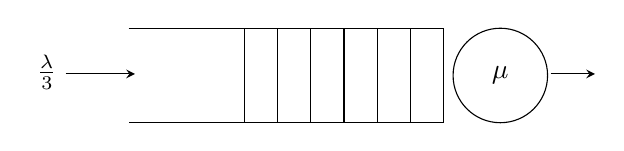
\begin{tikzpicture}[>=stealth, scale=0.8] 
            \draw (2,1.25) -- ++(5cm,0) -- ++(0,-1.5cm) -- ++(-5cm,0);
            \foreach \i in {1,...,6}
            \draw (7cm-\i*15pt,1.25) -- +(0,-1.5cm);
            \draw (7.9,0.5) circle [radius=0.75cm];
            \node[] at (0.7, 0.55) {$\frac{\lambda}{3}$};
            \draw[->] (1, 0.525) -- (2.1, 0.525);
            \node[] at (7.9,0.5) {$\mu$};
            \draw[->] (8.7,0.525) -- +(20pt,0);
        \end{tikzpicture}
    \end{figure}
    \begin{figure}[h]
        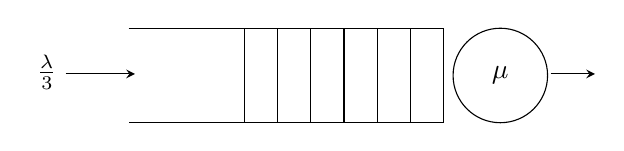
\begin{tikzpicture}[>=stealth, scale=0.8] 
            \draw (2,1.25) -- ++(5cm,0) -- ++(0,-1.5cm) -- ++(-5cm,0);
            \foreach \i in {1,...,6}
            \draw (7cm-\i*15pt,1.25) -- +(0,-1.5cm);
            \draw (7.9,0.5) circle [radius=0.75cm];
            \node[] at (0.7, 0.55) {$\frac{\lambda}{3}$};
            \draw[->] (1, 0.525) -- (2.1, 0.525);
            \node[] at (7.9,0.5) {$\mu$};
            \draw[->] (8.7,0.525) -- +(20pt,0);
        \end{tikzpicture}
    \end{figure}
    \begin{figure}[h]
        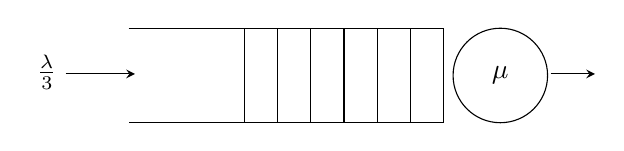
\begin{tikzpicture}[>=stealth, scale=0.8] 
            \draw (2,1.25) -- ++(5cm,0) -- ++(0,-1.5cm) -- ++(-5cm,0);
            \foreach \i in {1,...,6}
            \draw (7cm-\i*15pt,1.25) -- +(0,-1.5cm);
            \draw (7.9,0.5) circle [radius=0.75cm];
            \node[] at (0.7, 0.55) {$\frac{\lambda}{3}$};
            \draw[->] (1, 0.525) -- (2.1, 0.525);
            \node[] at (7.9,0.5) {$\mu$};
            \draw[->] (8.7,0.525) -- +(20pt,0);
        \end{tikzpicture}
    \end{figure}
\end{frame}

\begin{frame}
    \frametitle{Simulation - 3 servers}
    \centering
    \begin{figure}[h]
        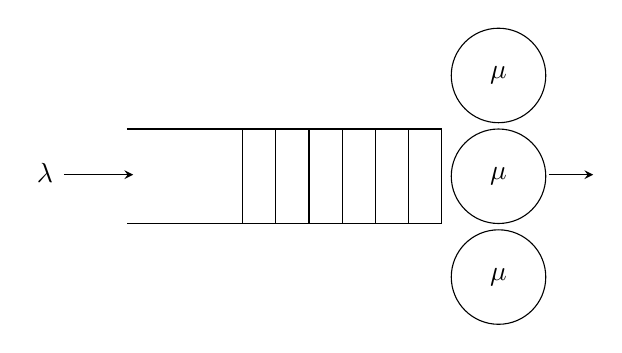
\begin{tikzpicture}[>=stealth, scale=0.8] 
            \draw (2,1.25) -- ++(5cm,0) -- ++(0,-1.5cm) -- ++(-5cm,0);
            \foreach \i in {1,...,6}
            \draw (7cm-\i*15pt,1.25) -- +(0,-1.5cm);
            \draw (7.9,-1.1) circle [radius=0.75cm];
            \node[] at (7.9,-1.1) {$\mu$};
            \draw (7.9,0.5) circle [radius=0.75cm];
            \node[] at (7.9,0.5) {$\mu$};
            \draw (7.9,2.1) circle [radius=0.75cm];
            \node[] at (7.9,2.1) {$\mu$};
            \node[] at (0.7, 0.55) {$\lambda$};
            \draw[->] (1, 0.525) -- (2.1, 0.525);
            \draw[->] (8.7,0.525) -- +(20pt,0);
        \end{tikzpicture}
    \end{figure}
\end{frame}


\begin{frame}
    \frametitle{Simulation - Queue with two waiting spaces}
    \centering
    \begin{figure}[h]
        \begin{tikzpicture}[>=stealth, scale=0.7] %arrow type
            % the rectangle with vertical rules (Queue 1)
            \draw (0,0) -- ++(2cm,0) -- ++(0,-1.5cm) -- ++(-2cm,0);
            \foreach \i in {1,...,4}
            \draw (2cm-\i*10pt,0) -- +(0,-1.5cm);
            
            % the circle (Queue 1)
            \draw (2.75,-0.75cm) circle [radius=0.75cm];
    
            % the rectangle with vertical rules (Queue 2)
            \draw (5,1.25) -- ++(2cm,0) -- ++(0,-1.5cm) -- ++(-2cm,0);
            \foreach \i in {1,...,4}
            \draw (7cm-\i*10pt,1.25) -- +(0,-1.5cm);

            % The two vertical lines at the very start of Queue 2 
            \draw (7cm-54pt,1.2) -- +(0,-0.5cm);
            \draw (7cm-54pt,0.3) -- +(0,-0.5cm);        
            \draw (7cm-51pt,1.1) -- +(0,-0.4cm);
            \draw (7cm-51pt,0.3) -- +(0,-0.4cm);
    
            % The label between the lines for T
            \node[anchor=north] at (5.15, 0.83 cm) {\scriptsize{T}};

            % the circle (Queue 2)
            \draw (7.75,0.5) circle [radius=0.75cm];
    
            % the arrows and labels (Queue 1+2)
            \draw[->] (8.5,0.525) -- +(20pt,0);
            \node[align=center] at (1cm,-2cm) {};
            \node[align=center] at (6cm,-0.75cm) {};
            
            % Ambulance lines
            \draw[<-] (0,-0.75) -- +(-50pt,0) node[left] {\( \lambda_2 \)};
            \draw[-] (3.5,-0.75) -- +(20pt,0);
            \draw (4.2, 0.525) -- (4.2, -0.75);

            % Others lines
            \draw (4.2, 1.8) -- +(-169.5pt,0) node[left] {\( \lambda_1 \)};
            \draw (4.2, 1.8) -- (4.2, 0.525);
            \draw[->] (4.2, 0.525) -- (5, 0.525);

        \end{tikzpicture}
    \end{figure}


\end{frame}